\chapter{A search for new phenomena}
\label{chapter:2ljets}

\begin{epigraphs}
\qitem{%
An experiment is never a failure solely because it fails to
achieve predicted results. An experiment is a failure only when it also
fails adequately to test the hypothesis in question, when the data it
produces don’t prove anything one way or another.%
}%
{Robert M. Pirsig~\cite{pirsig1999zen}}
\qitem{%
But there is one feature I notice that is generally missing in cargo cult
science. \ldots\
% That is the idea that we all hope you have learned in studying science in
% school--we never say explicitly what this is, but just hope that you catch
% on by all the examples of scientific investigation. It is interesting,
% therefore, to bring it out now and speak of it explicitly.
It's a kind of scientific integrity, a principle of scientific thought that
corresponds to a kind of utter honesty --- a kind of leaning over backwards.%
}%
{Richard Feynman~\cite{feynman1974cargo}}
\end{epigraphs}


Our central result is Figure~\ref{fig:2ljets_summary}, which shows the names,
data, and fitted background expectations with error bars in all main regions.
This figure illustrates the background-model part of a \clown{likelihood}
function which is extended with signals to test alternative models.
Exclusion contours testing the addition of C1N2 and GMSB signals to these
backgrounds are shown in Figure~\ref{fig:2ljets_contours}.
Interpretations of discovery region data are displayed in
Table~\ref{tab:2ljets_discovery}.


% summary plot

\begin{figure}[tp]
\centering
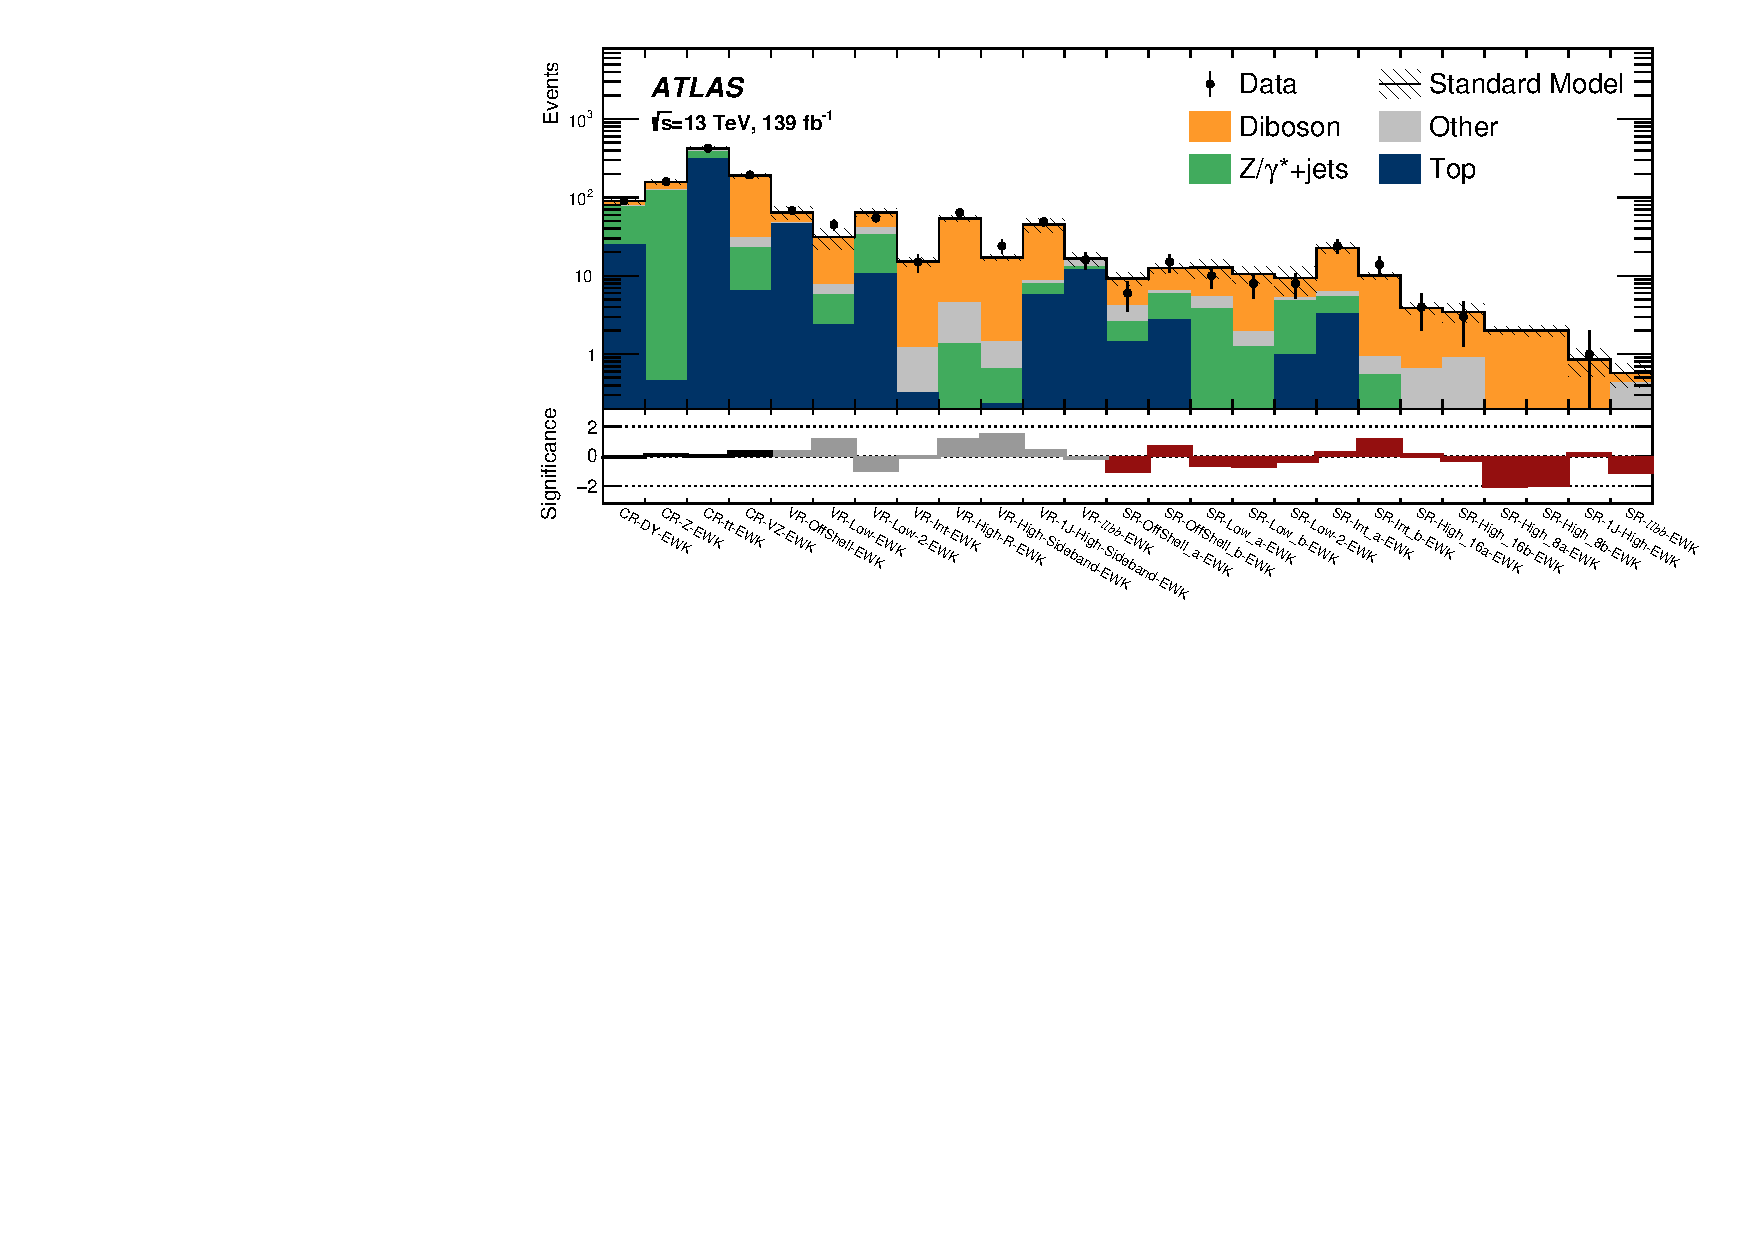
\includegraphics[width=\textwidth]{figures/2ljets_summary_log.pdf}
\caption{%
Data of the $\twoljets$ electroweak analysis with \emph{post-fit} backgrounds
for which the lower panel shows $S_\mathrm{ATLAS}$ from
Equation~\ref{eqn:significance_atlas}.
Control, validation and signal regions are shown from left to right, with the
regions within each category ordered approximately by their typical $\ptmiss$.
Likelihoods from validation regions are not included in the fit.
The `Top' category contains $t\bar t$ and $tW$ processes, and
`Other' contains fake/non-prompt lepton, higgs, triboson, $t\bar tZ$, and other
rare top processes.%
}
\label{fig:2ljets_summary}
\end{figure}


% exclusion plots

\begin{figure}[tp]
\centering
\begin{subfigure}{\textwidth}
    \centering
    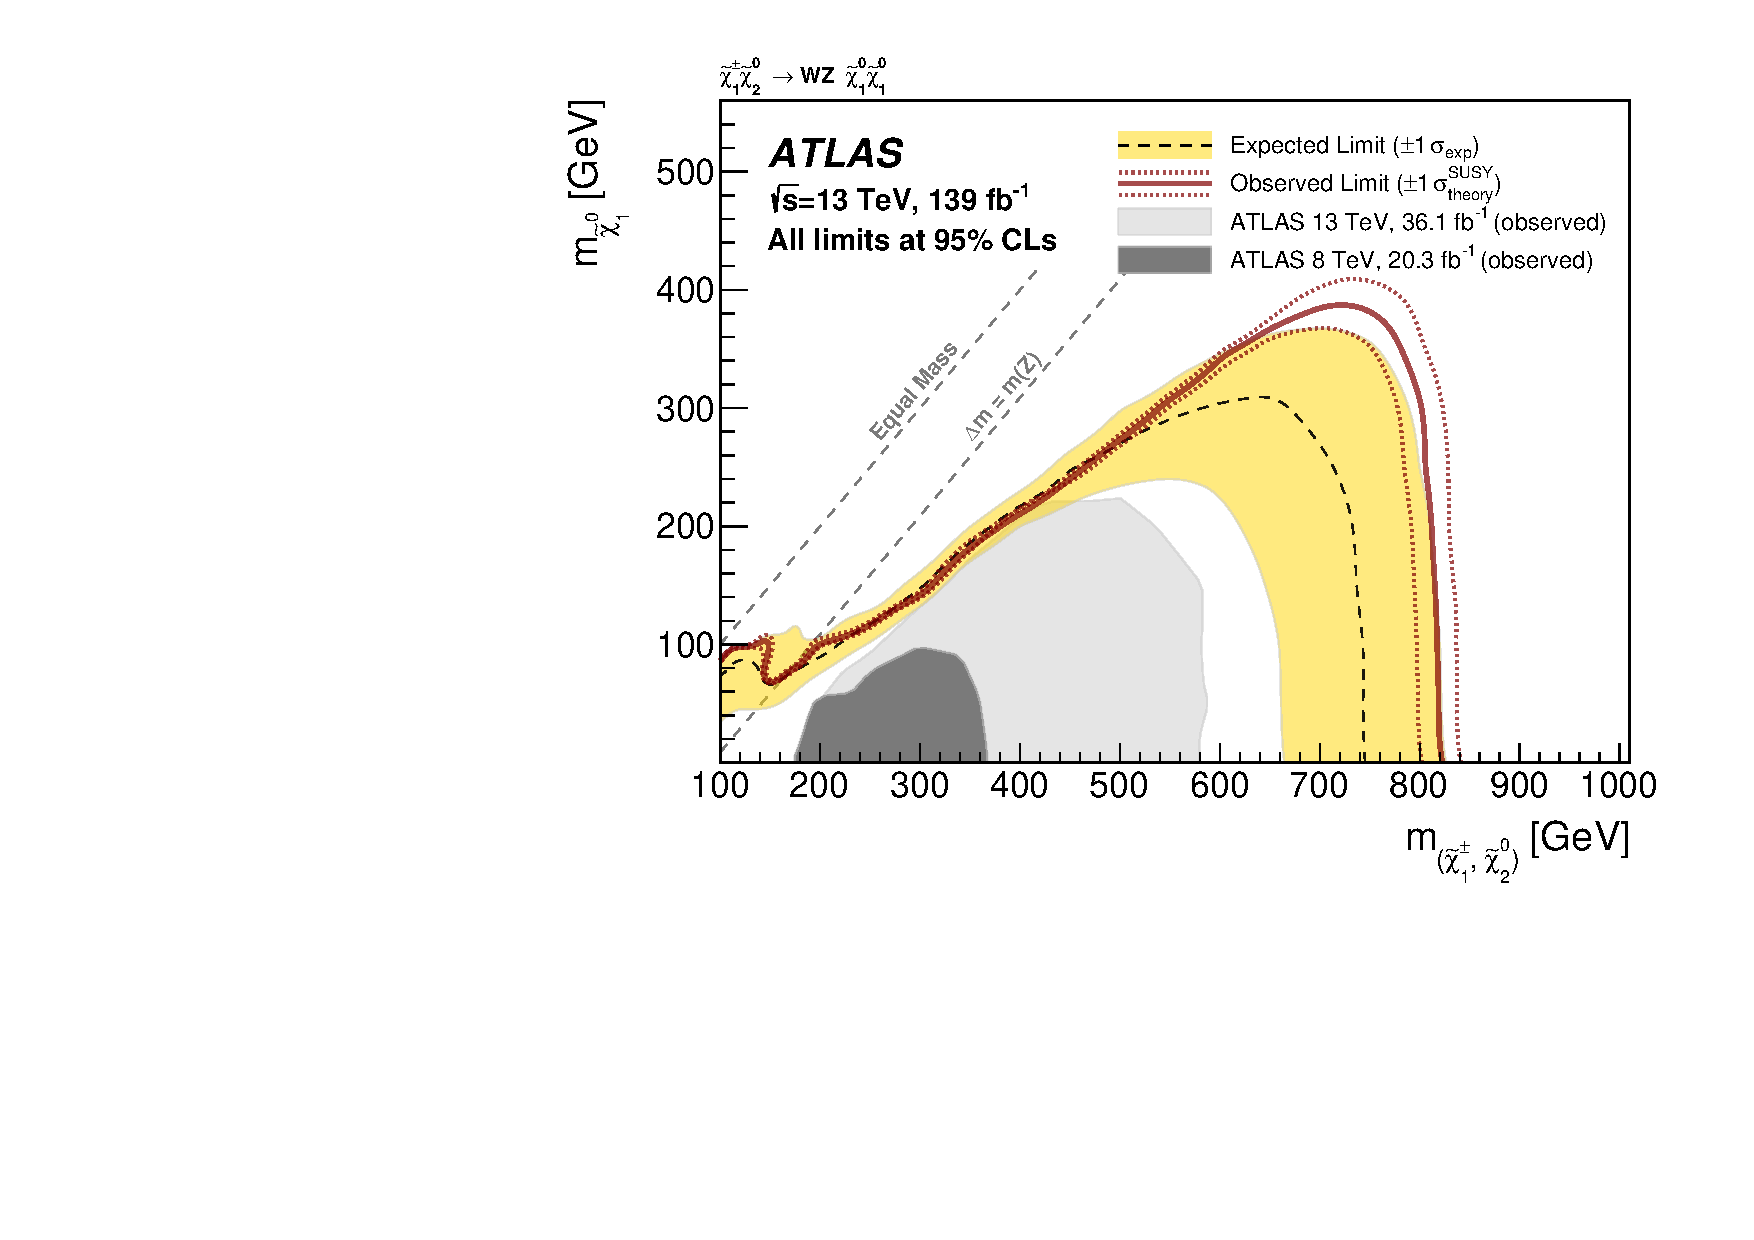
\includegraphics[width=0.7\textwidth]{figures/2ljets_contours_c1n2.pdf}
    \caption{C1N2 contours}
\end{subfigure}
\\[1em]
\begin{subfigure}{\textwidth}
    \centering
    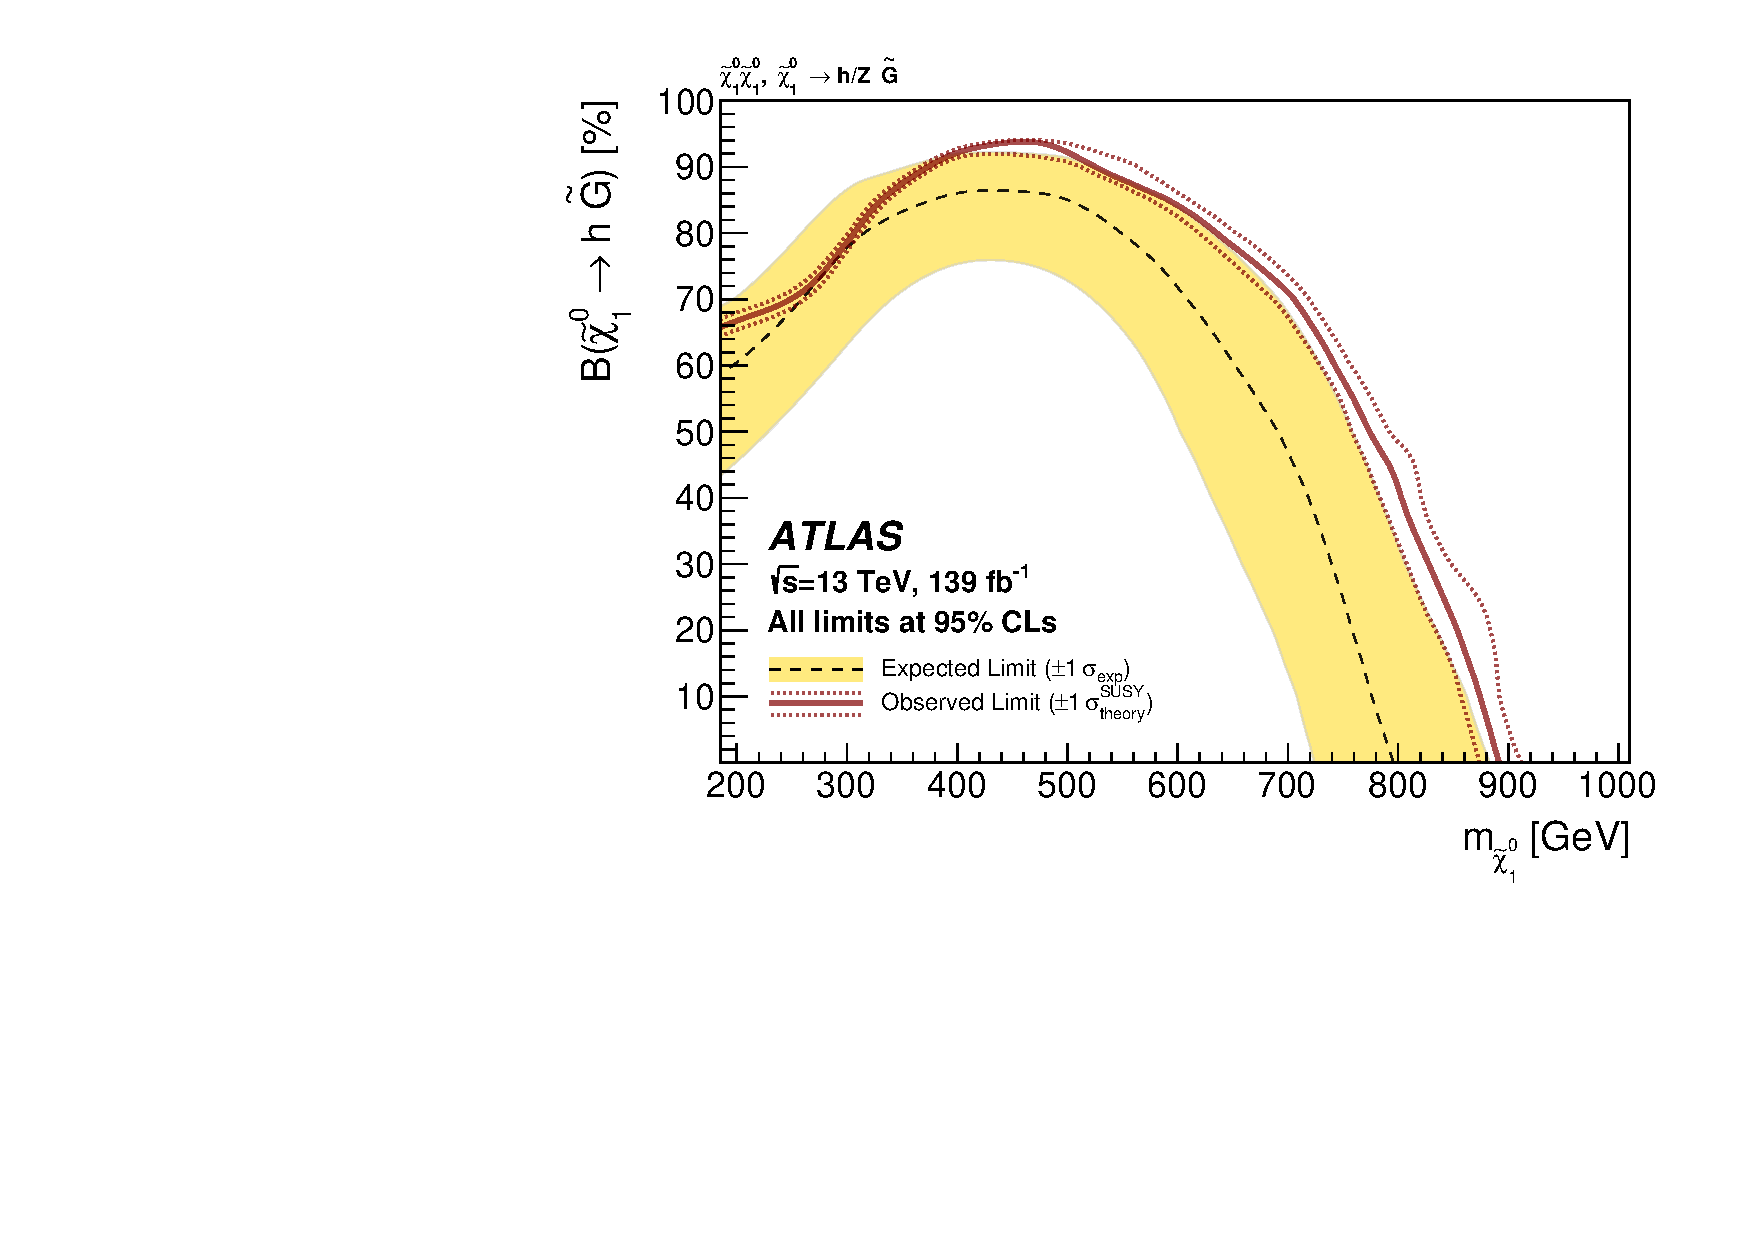
\includegraphics[width=0.7\textwidth]{figures/2ljets_contours_gmsb.pdf}
    \caption{GMSB contours}
\end{subfigure}
\caption{%
Contours from the $\twoljets$ electroweak analysis for
C1N2 (top) and GMSB (bottom) models.
Space below the solid red line is labelled as excluded and its dotted
neighbours show the result if all signal cross-sections are varied up and down
by theoretical error bars.
The yellow band shows the $\pm1$-sigma region of exclusion contours
from asymptotic approximations to the prior distribution of the test statistic.
Grey areas are observed limits from the two-lepton parts
of~\cite{SUSY-2016-24} and~\cite{SUSY-2013-11}.
Exclusion is defined by the $95\%$ $\mathrm{CLs}$ prescription
in asymptotic approximations.
All contours are interpolated from a sparse grid.
}
\label{fig:2ljets_contours}
\end{figure}


% upper limits
\begin{table}[tp]
\adjustbox{max width=0.98\textwidth}{%
\centering
\begin{tabular*}{\textwidth}{lccccccc}
{Region} &
\multicolumn{1}{c}{Fitted} &
\multicolumn{1}{l}{Data} &
$\langle A\epsilon{ \sigma}\rangle_{\mathrm{obs}}^{95}~\mathrm{fb}$ &
\multicolumn{1}{c}{$S_{\mathrm{obs}}^{95}$}  &
\multicolumn{1}{c}{$S_{\mathrm{exp}}^{95}$} &
$\mathrm{CLb}$ &
$p(s=0)~(Z)$  \\[1.5ex]
DR-OffShell      & $22.1\pm2.7$ & 21 & $0.10$ & $14.3$ & $12.3^{+4.7}_{-3.1}$ & $0.68$ & $0.50~(0.0)$ \\[.5ex]
DR-Low           & $22\pm4$ & 18 & $0.08$ & $10.8$ & $15.3^{+5.7}_{-4.0}$ & $0.09$ & $0.50~(0.0)$ \\[.5ex]
DR-Int           & $35\pm4$ & 38 & $0.15$ & $20.9$ & $17.5^{+5.9}_{-3.9}$ & $0.73$ & $0.23~(0.8)$ \\[.5ex]
DR-High          & $3.9\pm0.5$  & 0  & $0.02$ & $3.0$ & $5.6^{+2.2}_{-1.5}$ & $0.00$ & $0.50~(0.0)$ \\[.5ex]
DR-$\ell\ell bb$ & $0.51\pm0.20$  & 0  & $0.02$ & $3.0$ & $3.0^{+1.3}_{-0.0}$ & $0.19$ & $0.50~(0.0)$ \\[.5ex]
\end{tabular*}
}
\caption{%
Upper limit results in discovery region.
The fitted yield is in the background-only model constrained by the data in each region.
Limits are intended to reflect constrains on additive signal contributions.
\\[0.5em]
Left to right: the observed $95\%$ $\mathrm{CLs}$ upper limit on the visible cross-section
$\langle\epsilon\sigma\rangle_\mathrm{obs}^{95}$,
its corresponding signal expectation $S_\mathrm{obs}^{95}$,
expected $95\%$ upper limits on the signal expectation $S_\mathrm{exp}^{95}$
as would be obtained were the test statistic given by its central of $\pm 1$-sigma variations,
$\mathrm{CLb}$ evaluated with the signal expectation set to its observed upper limit,
and the discovery $p$-value capped at $0.5$ with its equivalent significance.
\\[0.5em]
Upper limits use the one-sided profile likelihood test statistic.
The discovery $p$-value uses a profile likelihood test statistic in a one-sided test.
All $p$-values are estimated by simulation of alternative data.
}
\label{tab:2ljets_discovery}
\end{table}
